% LaTeX source for ``Algorithms for Computer Simulation of Molecular Systems''
% Copyright (c) 2023 รังสิมันต์ เกษแก้ว (Rangsiman Ketkaew).

% License: Creative Commons Attribution-NonCommercial-NoDerivatives 4.0 International (CC BY-NC-ND 4.0)
% https://creativecommons.org/licenses/by-nc-nd/4.0/

\chapter{การคำนวณวิทยาศาสตร์สมรรถนะสูง}
\label{ch:high_perf_comp}

%----------------------------------------
\section{ทำไมต้อง High-Performance Computing ?}
%----------------------------------------

High-Performance Computing (HPC)คือเทคโนโลยีที่ใช้คลัสเตอร์คอมพิวเตอร์ (เครือข่ายของคอมพิวเตอร์หลาย ๆ เครื่องที่เชื่อมต่อและทำงานร่วมกัน)
ในการประมวลผลหรือคำนวณข้อมูลขนาดใหญ่และแก้ปัญหาทางคณิตศาสตร์ที่ซับซ้อนมาก ๆ ให้เสร็จในระยะเวลาที่เร็วที่สุด โดยทั่วไปแล้ว HPC
ทำงานหรือประมวลผลได้เร็วกว่าคอมพิวเตอร์ธรรมดาทั่วไปที่เราใช้ทำงานกันปกติหลายล้านเท่า\footnote{อ่านเพิ่มเติมเกี่ยวกับ HPC ได้ที่
  \url{https://www.ibm.com/topics/hpc}}

%----------------------------------------
\subsection{อัลกอริทึมสำหรับ Parallel Computing}
%----------------------------------------

ในปัจจุบันเราสามารถแบ่งอัลกอริทึมสำหรับการคำนวณ Parallel Computing ออกได้เป็น 2 อัลกอริทึม คือ Open Multi-Processing (OpenMP)
กับ Message Passing Interface (MPI) ซึ่งทั้งสองวิธีนี้มีความแตกต่างกันดังนี้

\paragraph{OpenMP}
เป็นวิธีที่เหมาะสำหรับการคำนวณกับหน่วยประมวลที่มีความเชื่อมโยงกันแบบแน่น (Tightly Coupled Multiprocessing) เช่น
เครื่องคอมพิวเตอร์ที่มีหน่วยประมวลผลหลาย ๆ ตัวอยู่ภายในเครื่องเดียวกันและมีการแชร์หน่วยความจำกัน (Shared Memory) โดยจะเป็นการใช้จำนวน
Threads หลาย ๆ ตัวมาใช้ในการวนลูปแบบขนานซึ่งเรียกว่า Fine Grain Parallelism (Loop Level) สำหรับการเขียนโค้ดเพื่อให้รันได้แบบ%
ขนานโดยการใช้ OpenMP สามารถทำได้ไม่ยาก เมื่อเทียบกับ วิธี MPI

\paragraph{MPI}
เป็นวิธีที่ตรงข้ามกับ OpenMP นั่นคือเหมาะสำหรับการคำนวณกับหน่วยประมวลผลที่มีความเชื่อมโยงกันแบบหลวม (Loosely Coupled Multiprocessing)
เช่น คลัสเตอร์หรือซุปเปอร์คอมพิวเตอร์ที่ประกอบไปด้วยคอมพิวเตอร์หลาย ๆ เครื่องที่เชื่อมต่อกันผ่านเครือข่ายภายใน (Local Network) วิธี MPI
มักถูกนำมาใช้สำหรับการทำ Coarse-Grain Parallelism (Domain Decomposition) การเขียนโค้ดเพื่อให้รันได้แบบขนานโดยการใช้ MPI
นั้นค่อนข้างมีความซับซ้อนมากกว่าการใช้วิธี OpenMP ขึ้นอยู่กับความเร็วของโค้ดที่เราต้องการให้เพิ่มขึ้น รวมไปถึงการออกแบบอัลกอริทึมสำหรับการแบ่ง
Workload ไปยัง Compute Node ต่าง ๆ และการ Communication ระหว่าง Node ด้วย

%----------------------------------------
\subsection{การเลือกใช้อัลกอริทึม Parallelism}
%----------------------------------------

ผมเชื่อว่าตอนนี้ผู้อ่านอาจจะเกิดคำถามว่าแล้วเราจะใช้ OpenMP หรือ MPI ในสถานการณ์ไหน ผมมีตัวอย่างมาให้ดู 3 กรณี จะได้เห็นภาพกันง่าย ๆ ครับ

\noindent \textbf{ตัวอย่างที่ 1}

\begin{quote}
  \color{gray}
  เราต้องการทำ Parallelization เพราะว่าหน่วยความจำของเครื่องที่ใช้รันโค้ดของเรานั้นไม่เพียงพอ เช่น เรามีการคำนวณที่มีความซับซ้อนมาก
  แล้วก็ขนาดของข้อมูลที่ใช้นั้นมีปริมาณเยอะมากซึ่งไม่สามารถ Fit กับขนาดของหน่วยความจำที่มี
\end{quote}

ในกรณีนี้เราควรใช้อัลกอริทึม MPI แล้วก็ควรจะเริ่มด้วยการใช้แค่ 1 MPI Process ต่อ 1 Compute Node ซึ่งจะเป็นการใช้หน่วยความจำให้ได้มากที่สุด

\noindent \textbf{ตัวอย่างที่ 2}

\begin{quote}
  \color{gray}
  เรามีข้อมูลที่มีปริมาณน้อยมากแล้วเราก็ต้องการแค่เพิ่มความเร็วของโค้ดที่กินทรัพยากรสิ้นเปลืองมาก ๆ ในการคำนวณ แล้วก็เราไม่อยากเสียเวลาในการทำ
  Parallelization
\end{quote}

ในกรณีนี้เราควรใช้อัลกอริทึม OpenMP เพราะว่าการเขียนโค้ด OpenMP นั้นทำได้ไม่ยากมาก เพียงแค่เขียนโค้ดเพิ่ม Statement เข้าไปแค่เพียงกี่บรรทัด
(ให้ครอบ Loop ที่เราต้องการทำ Parallel)

\noindent \textbf{ตัวอย่างที่ 3}

\begin{quote}
  \color{gray}
  เราต้องการเพิ่มหน่วยความจำเป็น (ใช้ Compute Node หลาย ๆ ตัว) แล้วก็ในขณะเดียวกันเราต้องการเพิ่มความเร็วในการคำนวณให้ได้มากที่สุดเท่าที่%
  จะเป็นไปได้ด้วย เช่น อยากให้โค้ดของเรารันด้วย Core หลาย ๆ Core ต่อ Compute Node
\end{quote}

ในกรณีนี้ค่อนข้างซับซ้อนกว่าตัวอย่างสองอันแรกสักหน่อย จากประสบการณ์ของผมพบว่าในกรณีข้างต้นนี้ Hardware มีบทบาทอย่างมากต่อประสิทธิภาพของ
Parallelization ถ้าหากว่าเครื่อง Compute Node ของเรามีจำนวน Core ที่ไม่เยอะ (เช่น 4-8 Cores) ประสิทธิภาพของการคำนวณจะขึ้นอยู่กับ
OpenMP (นั่นก็เพราะว่าโค้ดจะต้องมีการเริ่มต้น OpenMP Threads ก่อน) มากกว่าที่จะขึ้นกับ MPI (เพราะว่าการ Communication ระหว่าง Processors
ที่มีการแชร์หน่วยความจำร่วมกันนั้นไม่จำเป็นต้องใช้ MPI)

แต่ถ้าหากว่าเครื่อง Compute Node ของเรามีจำนวน Cores ที่เยอะ (เช่น 16 Cores ขึ้นไป) ในกรณีนี้เราควรใช้ Hybrid Algorithm ซึ่งเป็นการใช้
MPI และ OpenMP เพื่อมาทำ Parallelization แบบพร้อมกัน แต่ว่าการเขียนโค้ดให้รันได้ด้วย MPI และ OpenMP นั้นมีความยากมาก

%----------------------------------------
\section{ทักษะและเครื่องมือสำหรับการเขียนโปรแกรมสำหรับ HPC}
%----------------------------------------

\noindent \textbf{ทักษะที่จำเป็นในการทำความเข้าใจ HPC}

\noindent องค์ประกอบของ HPC
%
\begin{itemize}[topsep=0pt,noitemsep]
  \setlength\itemsep{0.5em}
  \item สถาปัตยกรรม (Architecture)

  \item การจัดการหน่วยความจำ (Memory Management)

  \item Kernels, Threading, Multithreading

  \item Block
\end{itemize}

\noindent อัลกอริทึมสำหรับการเขียนโค้ดแบบขนาน
%
\begin{itemize}[topsep=0pt,noitemsep]
  \setlength\itemsep{0.5em}
  \item Parallel Computing (SPMD)

  \item Shared Memory: OpenMP

  \item Distributed Memory: MPI

  \item Implementations: OpenMPI, Intel MPI, MVAPICH
\end{itemize}

\noindent คอมไพเลอร์ของ Intel
%
\begin{itemize}[topsep=0pt,noitemsep]
  \setlength\itemsep{0.5em}
  \item OpenMP Compiler: \inlinehighlight{icc}, \inlinehighlight{ifort}

  \item MPI Compiler: \inlinehighlight{mpicc}, \inlinehighlight{mpiicc} (สำหรับ Intel C Compiler),
        \inlinehighlight{mpicxx} (สำหรับ \cpp), \inlinehighlight{mpiifort} (สำหรับ Fortran)
\end{itemize}

\noindent \textbf{ทักษะสำหรับการเขียนโค้ดสำหรับ GPU}

\noindent มีความเข้าใจภาษา CUDA (Operation)
%
\begin{enumerate}[topsep=0pt,noitemsep]
  \setlength\itemsep{0.5em}
  \item สามารถระบุ (Declare) และจัดสรร (Allocate) หน่วยความจำของ Host และ Device ได้

  \item สามารถเริ่มต้น (Initialize) การสร้างข้อมูลของ Host ได้

  \item ถ่ายโอนข้อมูลจาก Host ไปยัง Device

  \item สามารถสั่งให้ Kernels หลาย ๆ ตัวทำงานได้

  \item ถ่ายโอนผลการคำนวณจาก Device กลับไปยัง Host
\end{enumerate}

%----------------------------------------
\section{การทำให้เกิดเมทริกซ์รูปทแยง (Matrix Diagonalization)}
\idxboth{การทำให้เกิดเมทริกซ์รูปทแยง}{Matrix Diagonalization}
%----------------------------------------

ในหัวข้อนี้ผู้อ่านจะได้ศึกษาการทำให้เกิดเมทริกซ์รูปทแยงหรือ Matrix Diagonalization (ผมขอเรียกสั้น ๆ ว่า MatDiag เพื่อความสะดวก)
ในการคำนวณแบบขนาน (Parallel Computing) สำหรับการคำนวณทางเคมีควอนตัม โดย MatDiag คือการดำเนินการ (Operation)
ทางพีชคณิตเชิงเส้นแบบหนึ่งซึ่งถูกใช้อย่างแพร่หลายโดยเฉพาะในงานวิจัยด้านการคำนวณทางวิทยาศาสตร์ แน่นอนว่าโปรแกรมทางเคมีควอนตัมนั้นก็ใช้
MatDiag เยอะมาก ๆ ซึ่งมีความซับซ้อนเชิงการคำนวณอยู่ที่ $O(n^3)$ ทำให้เกิดปัญหาคอขวดและทำให้การคำนวณของระบบที่มีขนาดใหญ่นั้นช้ามาก ๆ
เพื่อแก้ปัญหาดังกล่าวจึงได้มีการพัฒนาเทคนิคและไลบรารี่ที่จะเข้ามาช่วยเราในการทำ MatDiag ได้แบบขนาดหรือ Parallel ซึ่งช่วยให้การทำ
MatDiag เร็วขึ้นถึง 50\% เลยทีเดียว เริ่มต้นเรามีเมทริกซ์ที่มีขนาดใหญ่และสมาชิกส่วนใหญ่ของเมทริกซ์นั้นมีค่าไม่เท่ากับ 0 (Nonzero Elements)
ซึ่งเราจะเรียกเมทริกซ์ประเภทนี้ว่าเมทริกซ์แบบเต็ม (Full Matrix) หรือเมทริกซ์แบบแน่น (Dense Matrix) ก็ได้ โดยเราสามารถแทน Dense
Matrix ได้โดยใช้รูปแบบที่เรียกว่า Block Cyclic ในการทำการคำนวณแบบขนานด้วยวิธี Message-Passing Interface (MPI)
ซึ่งเป็นการกำหนดการกระจาย Dense Matrix ไปยังหน่วยประมวลผล (Processor) แต่ละตัวของเครื่องคำนวณ (Compute Node)
ในคลัสเตอร์คอมพิวเตอร์

\begin{figure}[htbp]
  \centering
  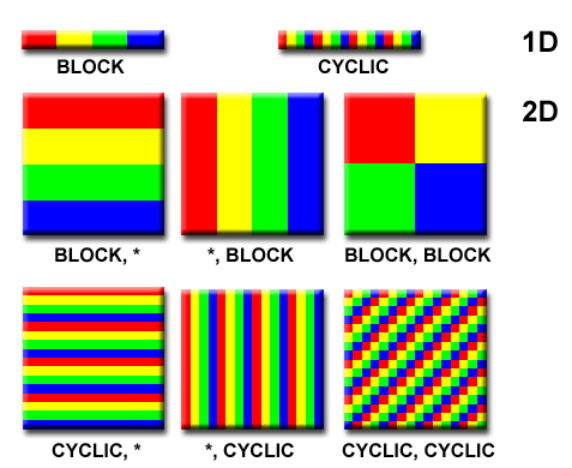
\includegraphics[width=0.7\linewidth]{fig/block_cyclic.png}
  \caption{เปรียบเทียบ Cyclic Format และ Block Format สำหรับการแสดงเวกเตอร์และเมทริกซ์ในการประมวลผลแบบขนาน (Parallel)
    ที่มีการใช้หน่วยประมวลผลหลายอัน (Multiple Processors) โดยแต่ละสีคือหน่วยประมวลผลที่แตกต่างกัน}
  \label{fig:block_cyclic}
\end{figure}

ให้ดูที่ภาพ \ref{fig:block_cyclic} ก่อนซึ่งเป็นการเปรียบเทียบการกระจายแบบ \enquote{Cyclic} และแบบ \enquote{Block}
สำหรับเวกเตอร์ 1 มิติและเมทริกซ์ 2 มิติ (ภาพด้านล่างผมคัดลอกมาจาก Tutorial \enquote{Introduction to Parallel} ของ Blaise
Barney แห่งสถาบัน LLNL) โดยสีแต่ละสีของแต่ละช่องนั้นจะเป็นการบ่งบอกถึง Processor ที่ต่างกัน และแต่ละ Segment นั้นจะบ่งบอกถึงสัดส่วน
(Portion) ของ Dense Matrix ที่ถูกกำหนดและแบ่งเข้าไปใน Local Memory ของแต่ละ Processor สำหรับการแยกออกเป็นส่วน ๆ แบบหมุนวน
(Cyclic Decomposition) ของเมทริกซ์นั้นสามารถทำได้คือเราจะทำการ Distribute แต่ละแถวหรือแต่ละคอลัมน์ไปยัง Processor ที่แตกต่างกัน
(เราอาจจะแบ่งเป็นทีละคู่ก็ได้ เช่น แบ่งทุก ๆ 2 แถว) ในทางตรงข้ามนั้น วิธีการแบ่งแบบ Block Representation นั้นจะเป็นการแยกเมทริกซ์%
ออกเป็นเมทริกซ์ย่อย ๆ จำนวน $N$ เมทริกซ์ (เรียกว่า Submatrices ก็ได้) โดยไม่สนใจว่าขนาดของแต่ละ Block นั้นจะต้องมีขนาดที่เท่ากัน
ซึ่งแต่ละ Submatrix นั้นจะถูกส่งต่อไปยัง Processor แต่ละตัว สรุปคือการแบ่งแบบ Cyclic นั้นเป็นการนำการแบ่งแบบ Block มาทำซ้ำ ๆ
กันไปแบบละเอียดกว่า ซึ่งจะทำให้เราได้ Block ที่มากกว่า

\begin{figure}[htbp]
  \centering
  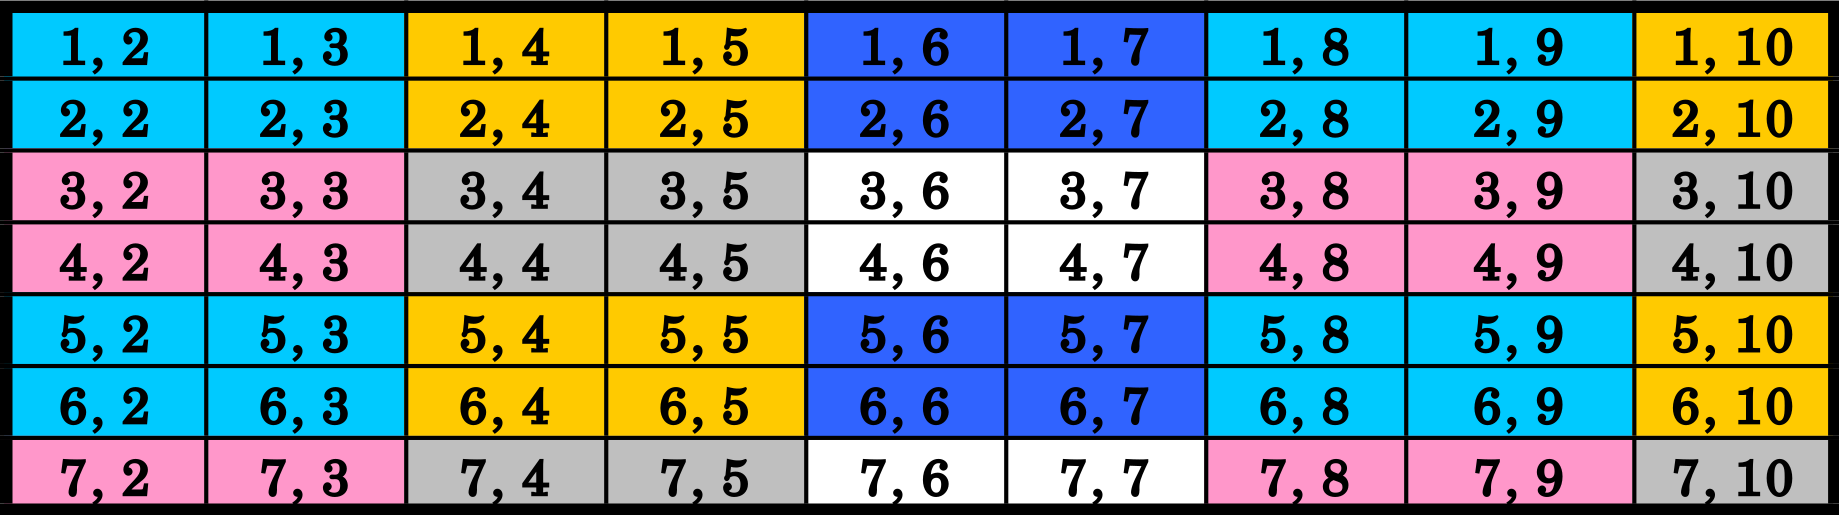
\includegraphics[width=0.7\linewidth]{fig/block_cyclic_matrix_global.png}
  \caption{Block Cyclic แบบ 2 มิติ: Global View}
  \label{fig:block_cyclic_matrix_global}
\end{figure}

\begin{figure}[htbp]
  \centering
  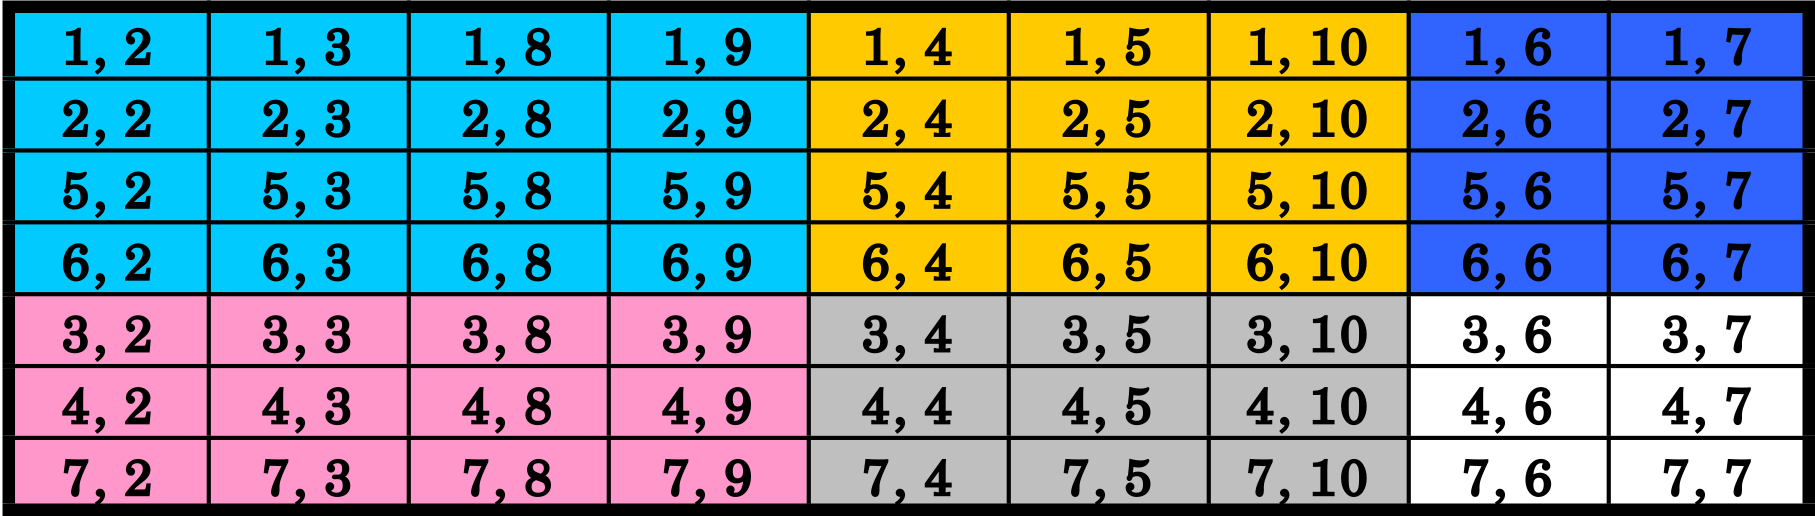
\includegraphics[width=0.7\linewidth]{fig/block_cyclic_matrix_local.png}
  \caption{Block Cyclic แบบ 2 มิติ: Local View}
  \label{fig:block_cyclic_matrix_local}
\end{figure}

แล้วข้อดีหรือข้อเสียของทั้งสองวิธีนี้คืออะไร? เราจะเห็นได้ว่า Cyclic Distribution นั้นจะเหมาะกว่าการกระจายเมทริกซ์แบบเท่า ๆ กัน (Evenly)
แต่ว่าจะมีการจัดการเมทริกซ์ที่ทำได้แย่กว่าเพราะว่าจะต้องมีการสื่อสาร (Communication) ระหว่าง Processor และระหว่าง Compute Node
ในการส่งต่อข้อมูลของ Matrix Element ที่ถูกคำนวณด้วย Processor ที่อยู่ใกล้กันซึ่งในทางตรงกันข้ามนั้นการ Communication ใน Block
Representation Matrix นั้นจะทำได้ดีกว่าเพราะว่ามันมีการแบ่งแบบต่อเนื่องบนหน่วยความจำ แต่ว่าถ้าหากว่า Matrix ของเราเป็นแบบ Sparse
Matrix หรือเมทริกซ์ที่มีสมาชิกส่วนใหญ่เป็น 0 นั้นก็อาจจะเกิดปัญหาเช่น Load Balancing ได้

\begin{figure}[htbp]
  \centering
  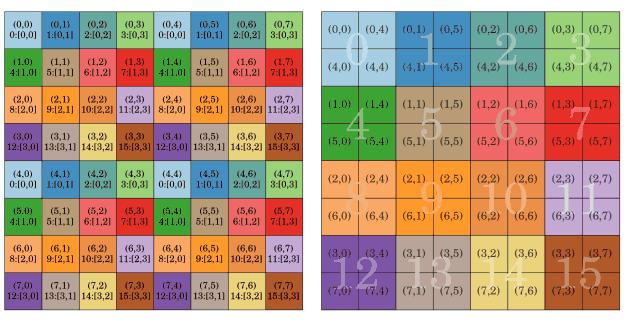
\includegraphics[width=0.7\linewidth]{fig/square_virtual_matrix.png}
  \caption{Square Virtual Matrix กับ Block Cyclic Distribution ด้านซ้ายคือ Global View ของการแบ่ง Array ตาม Block
    ด้านขวาคือ Local View ที่ข้อมูลนั้นถูกเก็บอยู่ในแต่ละหน่วยประมวลผลใน P-Array ส่วนตำแหน่งของ Process (Block Coordinates
    ในวงเล็บ) นั้นสอดคล้องกับ Linear Rank (Watermark)}
  \label{fig:square_virtual_matrix}
\end{figure}

เพื่อรวมข้อดีของทั้งสองวิธีไว้จึงได้มีการแบ่งแบบ Block Cyclic Distribution ซึ่งก็คือเป็นการแยกเมทริกซ์ออกเป็น Block เล็ก ๆ แล้วก็ทำการกระจาย
Blocks เหล่านี้แบบหมุนวน (Cyclically) ไปยัง Processors ทุกตัว โดยให้ดูตัวอย่างของ Block Cyclic Distribution ตามภาพที่
\ref{fig:block_cyclic_matrix_global} และ \ref{fig:block_cyclic_matrix_local}
สำหรับวิธีการแบ่งที่มีประสิทธิภาพที่สุดนั้นก็คือจำนวนของ Block ที่ถูกแบ่งออกมานั้นนั้นจะต้องเท่ากับจำนวนของ Processors
(หมายความว่ามีมิติเท่ากัน $N_{\text{row}} \times N_{\text{col}}$) โดย $N$ คือจำนวน Processors ซึ่งตามทั้งสองภาพนั้นเราจะเห็นได้ว่า
Block ที่มีสีเหมือนกันนั้นคือถูกคำนวณบน Processor เดียวกัน (ดู Local View) และขนาดของแต่ละ Block ควรจะต้องเท่ากันด้วย ส่วนภาพที่
\ref{fig:square_virtual_matrix} นั้นแถมให้ครับ ซึ่งก็เป็นอีกตัวอย่างของการแยกเมทริกซ์ออกเป็นส่วน ๆ (Decomposition) แบบ Block
Cyclic Distribution

%----------------------------------------
\section{การวัดประสิทธิภาพไลบรารี่สำหรับ Matrix Diagonalization}
%----------------------------------------

เราจะมาศึกษาการวัดประสิทธิภาพของไลบรารี่ ScaLAPACK กับ ELPA ซึ่งทั้งสองตัวนี้เป็นไลบรารี่สำหรับการทำ MatDiag แบบขนานซึ่งได้รับความนิยม%
ในการนำมาใช้ในการเขียนโปรแกรมที่รันบนซุปเปอร์คอมพิวเตอร์ เช่น โปรแกรมสำหรับการทำงานวิจัยด้านวิทยาศาสตร์ โดยเราได้ศึกษากันไปแล้วว่า%
ถ้าหากเรามี Dense Matrix $A$ ที่ถูกกระจายหรือแบ่งไปคำนวณบน Processors แต่ละตัวด้วยวิธี MPI โดยการใช้ Block Cyclic Distribution
สิ่งที่เรามักจะทำกันต่อจากนั้นก็คือการ Diagonalize ซึ่งเราต้องพยายามทำให้มัน Efficient ที่สุดโดยการทำ Diagonalization
นั้นคือการหาคำตอบของปัญหาค่าไอเกน (Eigenvalue Problem) ดังต่อไปนี้

\begin{equation}
  AX
  =
  XL
\end{equation}

\noindent โดยที่ $X$ คือเมทริกซ์ที่บรรจุ Eigenvector ของ $A$ ไว้ ส่วน $L$ นั้นคือเมทริกซ์ที่บรรจุค่า Eigenvalue ซึ่งเมทริกซ์ $L$
นี้เองที่เราจะต้องมาทำการหาเพราะมันเป็น Diagonal เมทริกซ์จริง ๆ ของ $A$

ในไลบรารี่ ScaLAPACK นั้นมีอัลกอริทึม 3 ตัวที่เราสามารถนำมาใช้ในการทำ Diagonalize Matrix ที่เป็น Real Symmetry Matrix
(เมทริกซ์ที่มีความสมมาตรและมีเพียงแค่ค่าจริงเป็นสมาชิกเท่านั้น) นั่นคือ \inlinehighlight{p?syevd}, \inlinehighlight{p?syevx},
และ \inlinehighlight{p?syevr} โดยที่ \inlinehighlight{?} นั้นแทนด้วยค่าที่บ่งบอกถึงประเภทของข้อมูลในเมทริกซ์ เช่น ถ้าแทน
\inlinehighlight{?} ด้วย \inlinehighlight{d} จะหมายถึงเมทริกซ์นั้นเก็บข้อมูลประเภท Double Precision หรือความเที่ยงแบบสองเท่า%
ซึ่งเป็นประเภทของข้อมูลแบบหนึ่งของ Floating Point หรือจำนวนจุดลอยตัว (ผมแนะนำว่าให้เรียกโดยการใช้คำศัพท์ภาษาอังกฤษไปเลย
เพราะว่าคำแปลภาษาไทยนั้นอาจจะเข้าใจได้ยากกว่า) โดยทั้งสามอัลกอริทึมนี้ก็จะใช้วิธีที่แตกต่างกันไป เช่น syevd จะใช้วิธีแบ่งแยกและเอาชนะ
(Divide and Conquer) ซึ่งผลการทดสอบที่แสดงด้านล่างนั้นได้มาจากการใช้ \inlinehighlight{p?syevd} นั่นเองครับ โดยสรุปสั้น ๆ คือวิธี
Divide and Conquer นั้นจะเริ่มด้วยการทำการลดรูปเมทริกซ์ (Reduction) $A$ ให้เป็น Tridiagonal Matrix ก่อนโดยใช้การแปลง
Householder หลังจากนั้นก็ทำการหา Tridiagonal Eigenvalue ด้วยอัลกอริทึม Divide and Conquer แล้วก็ทำการแปลงย้อนกลับไปให้ได้เป็น
Eigenvector ออกมา

ตามที่ผมได้อธิบาย \inlinehighlight{p?syevd} ของไลบรารี่ ScaLAPACK ไปแล้วนั้น ลำดับต่อไปคือไลบรารี่ยอดฮิตอีกตัวที่ได้รับความนิยมใน%
การนำมาใช้ในโปรแกรมทางเคมีควอนตัมหลายตัวด้วยกัน เช่น NWChem และ CP2K นั่นก็คือไลบรารี่ ELPA จริง ๆ แล้ว ELPA นั้นเอาอัลกอริทึมใน
ScaLAPACK มาปรับปรุงอีกทีนึงเพื่อให้มีประสิทธิภาพมากขึ้น โดยจะใช้เทคนิค Direction Transformation ของ Tridiagonal Form
ซึ่งก็มีความซับซ้อนพอสมควร เอาเป็นว่าทั้ง ScaLAPACK กับ ELPA ก็สามารถนำมาใช้ได้ทั้งคู่ แล้วก็ Interface นั้นมีความคล้ายคลึงกันมาก
สิ่งที่แตกต่างอีกอย่างหนึ่งก็คือ ELPA นั้นมีความ General มากกว่าตรงที่สามารถใช้กับ Fortran Kernel ได้บนหลากหลายสถาปัตยกรรมมากกว่า
เช่น ถ้า Kernel ของ CPU เป็นแบบใหม่ ๆ เช่น AVX, AVX2, หรือ AVX-512 นั้น ELPA ก็จะรองรับ คราวนี้เรามาดูการทำ Benchmark
หรือการวัดประสิทธิภาพของไลบรารี่ทั้งคู่นี้กัน ปกติแล้วการทำ MatDiag นั้นจะขึ้นอยู่กับปัจจัยหลายตัว โดยหลัก ๆ แล้วมีดังนี้

\begin{enumerate}[topsep=0pt,noitemsep]
  \setlength\itemsep{0.5em}
  \item ขนาดของ Matrix

  \item โครงสร้างของ Matrix

  \item จำนวน Processors ของเครื่องที่ใช้ในการรันหรือคำนวณ Diagonalization

  \item ขนาดของ MPI Block Size สำหรับ Matrix

  \item อัลกอริทึมที่ใช้ในการทำ Diagonalization
\end{enumerate}

\begin{figure}[htbp]
  \centering
  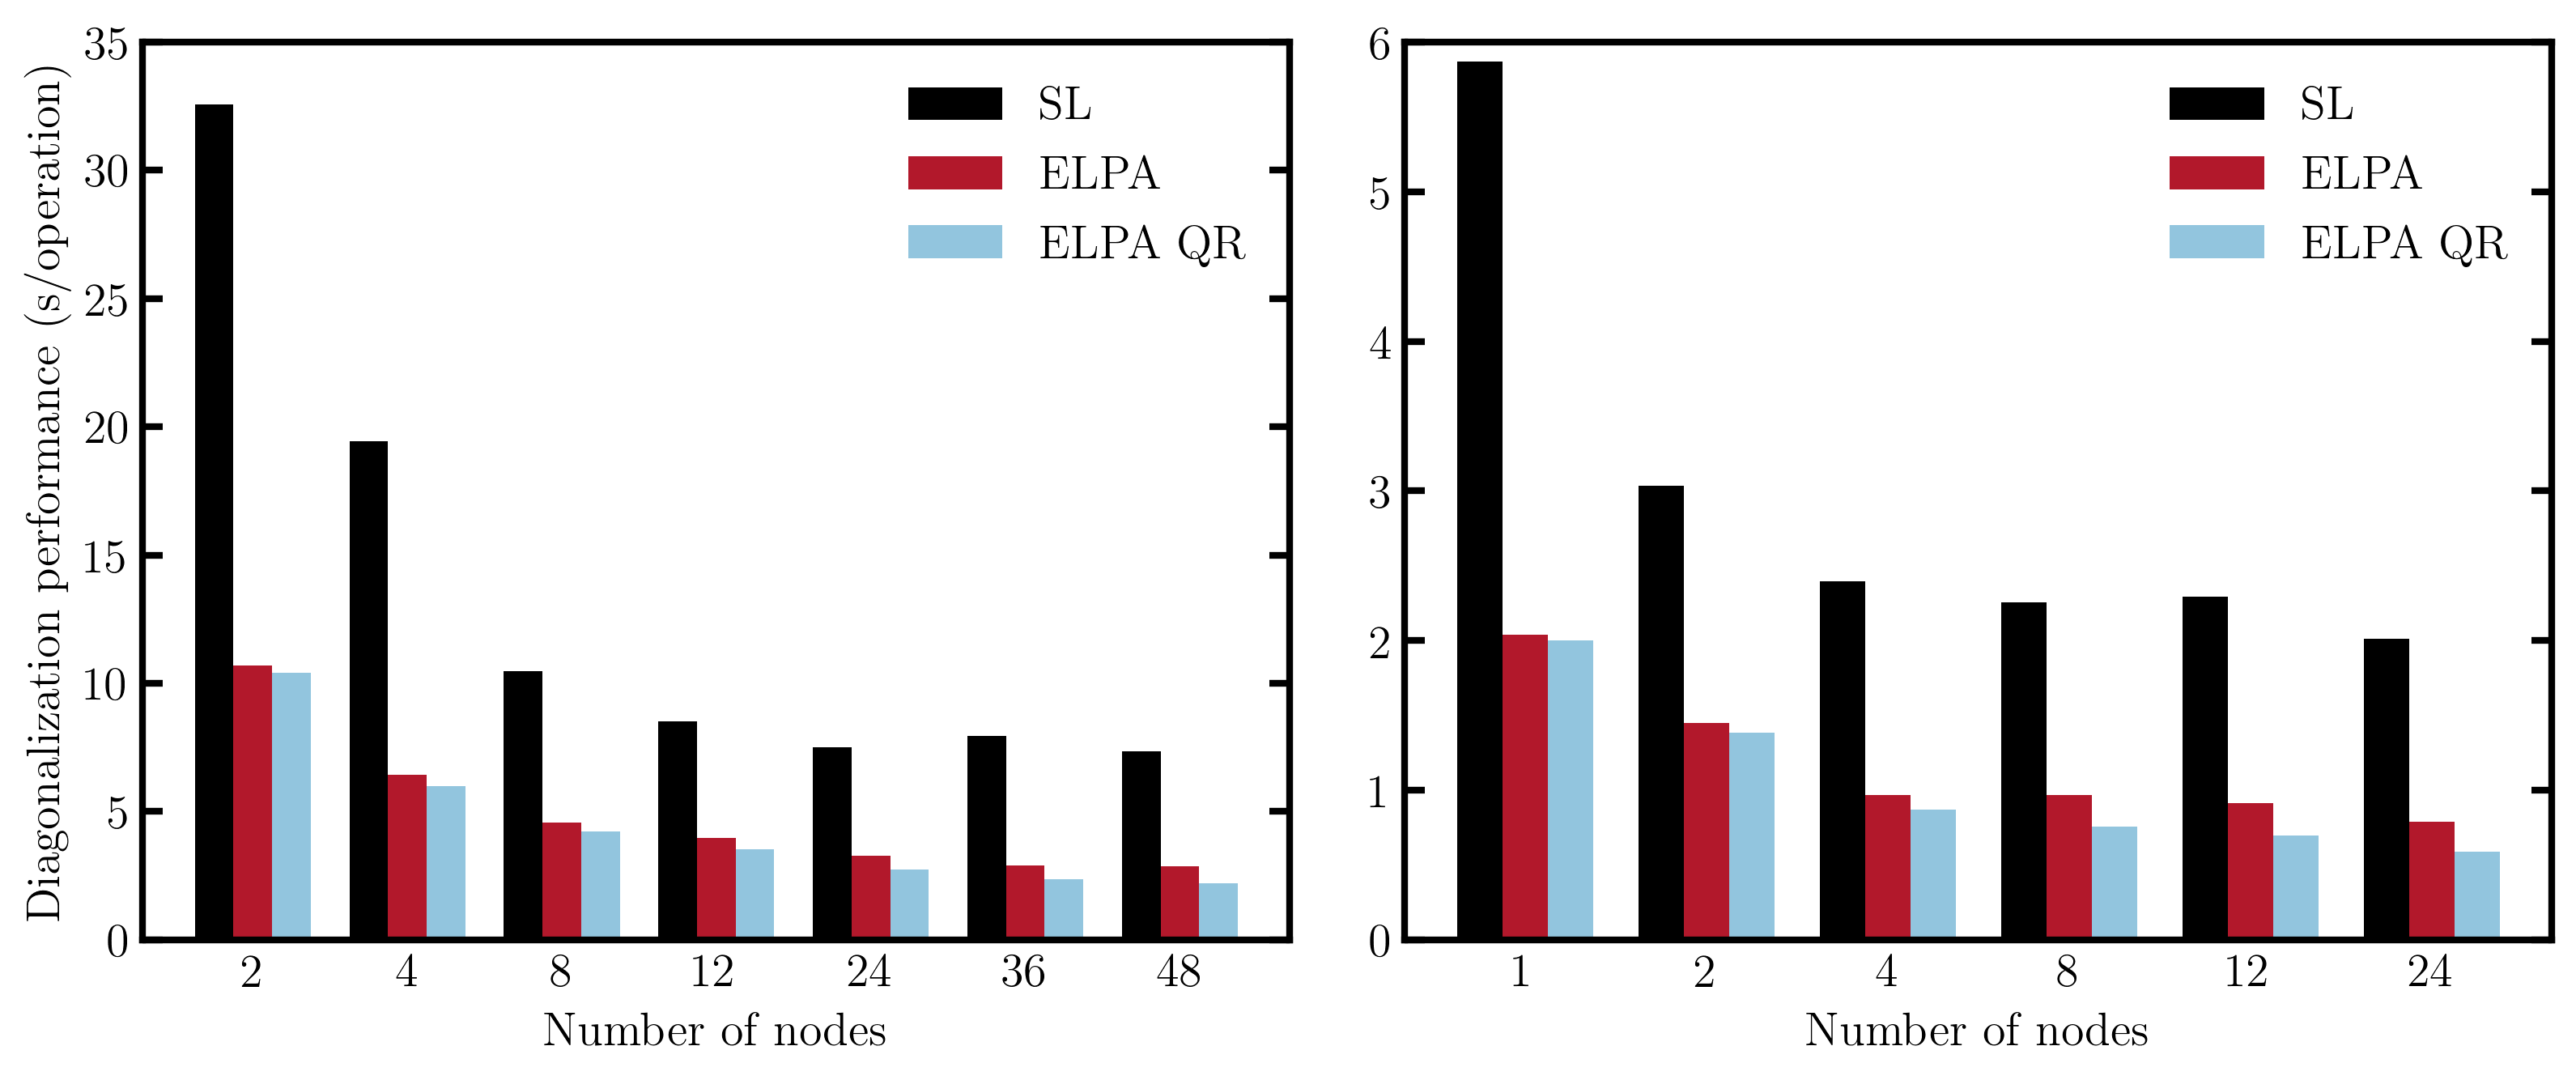
\includegraphics[width=0.8\linewidth]{fig/diag_perf.png}
  \caption{Local View}
  \label{fig:diag_perf}
\end{figure}

สำหรับตัวอย่างที่เราจะมารันทดสอบ Benchmark กันนัั้นก็คือเมทริกซ์จตุรัสขนาด $5888 \times 5888$ กับขนาด $13034 \times 13034$
ตามลำดับ โดยใช้โปรแกรม CP2K (โปรแกรมทางเคมีควอนตัม) ซึ่งจริง ๆ แล้วก็คือระบบที่เป็นโมเลกุลน้ำ (Water Cluster) 128 โมเลกุลนั่นเอง
สำหรับเครื่องซุปเปอร์คอมพิวเตอร์ที่ใช้ในการทดสอบนั้นคือ Cray XC40 ซึ่งมีสเปคคือแต่ละโหนดนั้นจะมี 12-core Intel Xeon E5-2690v3 Processors
ทั้งหมด 2 ตัว และมี Memory คือ 64 GB (DDR4) สำหรับผลการทดสอบนั้นก็ดูได้ตามภาพที่ \ref{fig:diag_perf} ได้เลย แกน y
คือประสิทธิภาพที่ได้ส่วนแกน $x$ นั้นคือจำนวนของ Node ของ Cray XC40 โดย SL คือ ScaLAPACK, ส่วน QR นั้นคือเทคนิค Decomposition
แบบหนึ่งที่เราเอาเข้ามาช่วยในการเพิ่มประสิทธิภาพการทำ Diagonalization ของ ELPA นั่นเอง ภาพด้านซ้ายคือระบบที่เมทริกซ์ขนาดใหญ่
ส่วนภาพด้านขวาเมทริกซ์ขนาดเล็ก สรุปคือจากการทดสอบนั้นก็คือ ELPA ชนะขาดลอยในการทำ Diagonalization แบบขนานด้วย MPI ซึ่ง ELPA
ทำประสิทธิภาพได้ดีกว่า SL ประมาณ 60-80\% เลยทีเดียว

%----------------------------------------
\section{การประยุกต์ใช้ Matrix Diagonalization}
%----------------------------------------

หนึ่งในการประยุกต์ใช้ Matrix Diagonalization ในโปรแกรมเคมีเชิงคำนวณก็คือการคำนวณพลังงานของออร์บิทัล (Orbital Energies)
ซึ่งเป็นเทอมที่สำคัญมาก ๆ ในทางเคมีเพราะว่าเป็นตัวที่เราจะนำมาใช้ในการศึกษาโมเลกุล โดยหลาย ๆ คนที่เคยวิชาเคมีอินทรีย์เชิงฟิสิกส์มานั้นก็น่า%
จะเคยผ่านการใช้ H\"{u}ckel Model Theory ในการคำนวณหาพลังงานของออร์บิทัลของโมเลกุลเคมีอินทรีย์ (สารประกอบไฮโดรคาร์บอน) แบบง่าย ๆ
กันมาแล้ว เช่น โมเลกุลเบนซีน ซึ่งวิธีที่เราจะใช้ในการคำนวณหา Orbital Energy นั้นเราจะต้องทำการกำหนดฟังก์ชันคลื่นที่ใช้อธิบาย MO สำหรับ
$\pi$ Electron ขึ้นมาก่อน ซึ่งเราสามารถใช้ผลรวมเชิงเส้นของ Atomic Orbitals ได้ เช่น สำหรับโมเลกุลเบนซีน เขียนได้ดังนี้

\begin{equation}
  \phi_{n} = \sum_{i=1}^{6} C_{i} \chi_{i}
\end{equation}

\noindent โดยที่ $C_{i}$ คือ Molecular Orbital Coefficients และ $\chi$ คือ Basis Function คราวนี้เราสามารถใช้สมการ
Eigenfunction

\begin{equation}
  HC = \epsilon C
\end{equation}

\noindent ในการหา $\epsilon$ ซึ่งเป็นพลังงานของแต่ละออร์บิทัลได้ โดยที่ H คืออินทิกรัลของ Basis Function โดยหน้าตา H, C และ
$\epsilon$ นั้นจริง ๆ แล้วก็คือ Square Matrix ดี ๆ นี่เอง โดยสามารถดูตัวอย่างของทั้งสามเมทริกซ์นี้สำหรับกรณีโมเลกุลเบนซีนได้ตามภาพที่ 1
โดย $\alpha$ กับ $\beta$ นั้นก็คือ Coefficient ของแต่ AO แต่ละอันนั่นเอง เช่น อะตอมคาร์บอนตัวที่ 1 นั้นก็จะมี Interaction
กับคาร์บอนที่ 2 กับ 6 ซึ่งการแก้สมการ Secular Equation นี้เราสามารถทำ Diagonalization ได้ โดยจัดรูปสมการเป็น%
\footnote{ต้องทำความเข้าใจกันก่อนว่าทฤษฎี H\"{u}ckel Model นั้นจะ Treat หรือสนใจเฉพาะ MO ของ $\pi$ Electron สำหรับโมเลกุล%
ที่เป็นแบบ $\pi$-conjugated เท่านั้น}

\begin{equation}
  (H - \epsilon)C = 0
\end{equation}

หนึ่งในวิธีที่หลายคนมักจะนำมาใช้ในการทำ Diagonalization นั้นก็คือ Jacobi Method แต่ว่าวิธีนี้มีจุดอ่อนคือมันไม่ได้ทำการแยกตัวประกอบของ
Secular Equation ออกเป็นเทอม ๆ จึงทำให้เราไม่มี Main-diagonal Block แล้ว Main-diagonal Block คืออะไร? ทำไมถึงสำคัญ?
ประเด็นก็คือการที่เราทำ Diagonalization นั้นมันจะมีวิธีบางอย่างที่สามารถจัดการเมทริกซ์ให้อยู่ในรูปที่เกิดจากการประกอบกันระหว่าง Diagonal
Matrix หลาย ๆ อันได้และสมาชิกของเมทริกซ์ที่อยู่นอก Main-diagonal Block นั้นจะต้องเป็น 0 ด้วย เช่นให้ดูตามภาพที่ 2 ถ้าใครยังไม่เข้าใจ%
ให้ดูภาพที่ 3 จะได้เห็นภาพของ Diagonal Block ชัดขึ้น ซึ่งกลับมาที่ Jacobi Method ที่ไม่ได้ทำการแยก Block Diagonal Matrix
ออกมาให้เรา ซึ่งนี่เป็นสาเหตุที่ทำให้ Symmetry ของโมเลกุลนั้นหายไประหว่างการทำ Diagonalization และทำให้ออร์บิทัลที่เป็นแบบ Degenerate
(ออร์บิทัลที่มีพลังงานเท่ากัน) นั้นหายไปด้วย ซึ่งในความเป็นจริงโมเลกุลเบนซีนจะต้องมีบางออร์บิทัลที่มีพลังงานเท่ากัน ตามภาพที่ 4
ดังนั้นสิ่งที่เราต้องการคือ Diagonalization Method ที่สามารถให้ Main-diagonal Block ที่มีให้ Degenerate MOs อย่างไรก็ตามในการ%
คำนวณทางเคมีควอนตัมนั้นถ้าหากเราใช้ทฤษฎีอื่น ๆ นั้นก็จะมีการนิยามและคำนวณหาพลังงาน MO (Eigenvalues) ที่แตกต่างกันไปและซับซ้อนมากขึ้น
แต่หลัก ๆ แล้วก็จะต้องมีการทำ Diagonalization อยู่ดีครับ

%----------------------------------------
\section{การวัดประสิทธิภาพโปรแกรม \textit{ab initio} Molecular Dynamics}
%----------------------------------------

ในหัวข้อนี้เราจะมาดูรายละเอียดขั้นตอนการประเมินประสิทธิภาพ (ความเร็ว) ของโปรแกรม Ab initito Molecular Dynamics (AIMD) กันครับ
ในปัจจุบันนั้นมีโปรแกรมที่สามารถรันการคำนวณ AIMD หลายโปรแกรมมาก ๆ โดยโปรแกรมที่ได้รับความนิยม เช่น CPMD, Quantum Espresso,
CP2K, NWChem, VASP โดยส่วนตัวของผมเองนั้นก็ได้มีโอกาสวัดประสิทธิภาพ (Benchmarking) ความเร็วโปรแกรมที่กลุ่มวิจัยที่ผมมาศึกษาต่อนั้นใช้
ก็คือโปรแกรม CP2K ว่าทำงานได้เร็วและมี Speed-Up Scaling มากน้อยแค่ไหนบน Distributed System ของ Supercomputer

แน่นอนว่าขั้นตอนเริ่มต้นนั้นก็คือการเตรียมโครงสร้างของระบบโมเลกุลที่ต้องการนำมาใช้ในการทดสอบ แล้วก็รัน Simulation โดยการเปลี่ยนจำนวนของ
Compute Nodes โดยเริ่มจาก 1 Node และเพิ่มจำนวนเป็น 2, 4, 8, 16, 24, 32, 48, 64 Node เป็นต้น ซึ่งตามทฤษฎีแล้วนั้นความเร็วของ
Software ที่ได้ควรจะต้องเร็วขึ้นตามจำนวนเท่าของการเพิ่มจำนวน Compute Node

\begin{figure}[htbp]
  \centering
  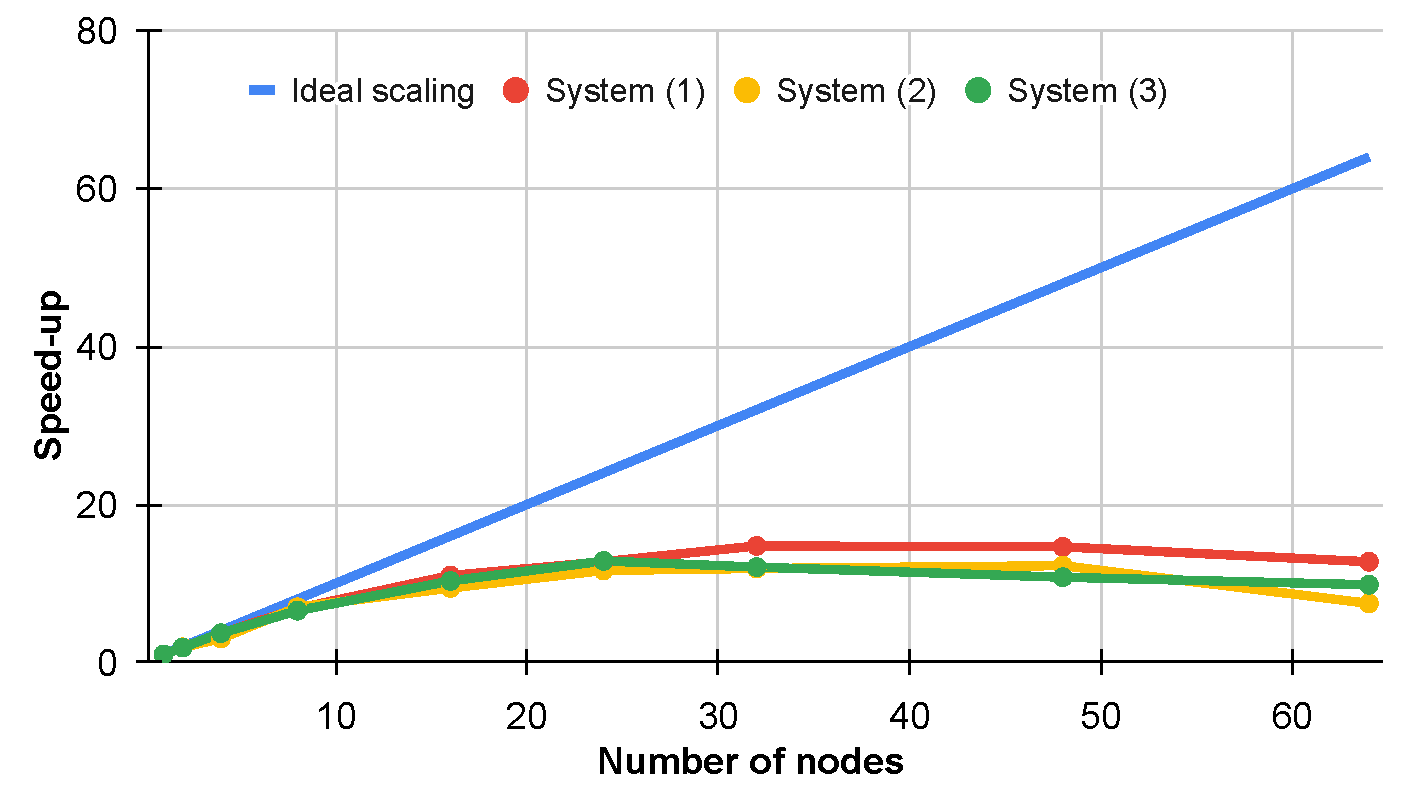
\includegraphics[width=0.9\linewidth]{fig/perf-scaling-cp2k.pdf}
  \caption{Speed-Up Scaling ของโปรแกรม CP2K ตามจำนวน Compute Nodes ของซุปเปอร์คอมพิวเตอร์ CSCS Piz Daint}
  \label{fig:perf_scaling_cp2k}
\end{figure}

แต่ในความจริงนั้นโปรแกรมของเราไม่ได้ทำงานเร็วตามทฤษฎีและ Speed-Up Scaling ก็ไม่ได้เป็น Linear Scaling หรอกครับ
มันมีปัญหาเยอะและมีหลายเหตุผลที่ทำให้เกิดคอขวด (Bottleneck) โดย Scaling ที่ได้ก็ตามกราฟในรูปที่ \ref{fig:perf_scaling_cp2k}
จะเห็นว่าพอเราเพิ่มจำนวน Compute Node จาก 24 $\rightarrow$ 32 แล้ว Efficiency (คำนวณจาก Speedup หารด้วยจำนวน Node)
เริ่มลดลง

คำถามคือสิ่งที่ผมทำนี้มันถูกต้อง 100\% ไหม จริง ๆ แล้วไม่ถูก 100\% เพราะว่าการที่เรารัน MD Simulation หลาย ๆ ครั้งถึงแม้ว่าจะใช้ Input
ไฟล์เดียวกันและเหมือนกันทั้งหมดนั้น สิ่งที่เกิดขึ้นคือผลการคำนวณที่ได้จะไม่มีทางที่เหมือนกัน นั่นก็เพราะว่าอัลกอริทึมของโปรแกรม MD
(เรียกได้ว่าเกือบทุกโปรแกรมเลย) จะมีการสุ่ม (Random) พารามิเตอร์บางตัวขึ้นมาก่อนใน Step แรกสุดของการคำนวณ
ซึ่งพารามิเตอร์นั้นก็คือความเร็วของอะตอมแต่ละตัวในโมเลกุลซึ่งจะถูกนำมาใช้ในการแก้สมการ Newton แบบคลาสสิคสำหรับการคำนวณหาแรง (Force)
เพื่อใช้ในการอัพเดทตำแหน่งของอะตอมแต่ละตัวใน Step ต่อไป ซึ่งเราเรียกเท่ ๆ ว่าการ Propagation
(ใน CP2K เราใช้ DFT-MD ซึ่งจะใช้ควอนตัมในการคำนวณพลังงานและแรงของอะตอมแต่ละตัว ซึ่งเรามักจะ \enquote{เคลม}
และเชื่อว่าให้ผลที่แม่นยำและถูกต้องกว่าใช้ Force Field)

ถึงแม้ว่าเราจะรัน Simulation ด้วยไฟล์ Input เดียวกัน 2 รอบ ผลการคำนวณนั้นจะไม่เหมือนกัน เช่น พลังงานของระบบในแต่ละ MD Step
นั้นถ้าเทียบกันแล้วจะแตกต่างกันอย่างสิ้นเชิง และแน่นอนว่าระยะเวลาจริงที่ใช้ในการคำนวณ (Simulation Time) ของแต่ละ MD Step นั้นก็ต่างกันด้วย
เหตุผลก็ตามที่ได้บอกไปคือ Initial Parameter นั้นไม่เหมือนกัน จึงทำให้การรันสองทั้งนั้นให้ผลที่ไม่เหมือนกัน

ถ้าถามว่าผิดไหมที่โปรแกรม MD ส่วนใหญ่นั้นทำการสุ่มค่าความเร็วเริ่มต้นของอะตอมแต่ละตัว คำตอบคือไม่ผิด เพราะว่าท้ายที่สุดแล้วเราสนใจระบบกรณี%
ที่มีความเป็น Ergodicity แบบสมบูรณ์แล้ว เมื่อเรารัน Simulation ไปเรื่อย ๆ จนระบบเข้าสู่สภาวะสมดุล (Equilibrium) เราสามารถอ้างได้ว่า
Configuration แต่ละตัวนั้นสามารถที่จะ Represent คุณสมบัติแบบ Microscopic ได้

\vspace{5pt}

\begin{lstlisting}[
  style=MyFortran,
  basicstyle=\ttfamily\footnotesize\linespread{0.5}
  ]
DO i = 1, natoms
  atomic_kind => part(i)%atomic_kind
  CALL get_atomic_kind(atomic_kind=atomic_kind, mass=mass)
  part(i)%v(1) = 0.0_dp
  part(i)%v(2) = 0.0_dp
  part(i)%v(3) = 0.0_dp
  IF (mass .NE. 0.0) THEN
     SELECT CASE (is_fixed(i))
     CASE (use_perd_x)
        part(i)%v(2) = globenv%gaussian_rng_stream%next()/SQRT(mass)
        part(i)%v(3) = globenv%gaussian_rng_stream%next()/SQRT(mass)
     CASE (use_perd_y)
        part(i)%v(1) = globenv%gaussian_rng_stream%next()/SQRT(mass)
        part(i)%v(3) = globenv%gaussian_rng_stream%next()/SQRT(mass)
     CASE (use_perd_z)
        part(i)%v(1) = globenv%gaussian_rng_stream%next()/SQRT(mass)
        part(i)%v(2) = globenv%gaussian_rng_stream%next()/SQRT(mass)
     CASE (use_perd_xy)
        part(i)%v(3) = globenv%gaussian_rng_stream%next()/SQRT(mass)
     CASE (use_perd_xz)
        part(i)%v(2) = globenv%gaussian_rng_stream%next()/SQRT(mass)
     CASE (use_perd_yz)
        part(i)%v(1) = globenv%gaussian_rng_stream%next()/SQRT(mass)
     CASE (use_perd_none)
        part(i)%v(1) = globenv%gaussian_rng_stream%next()/SQRT(mass)
        part(i)%v(2) = globenv%gaussian_rng_stream%next()/SQRT(mass)
        part(i)%v(3) = globenv%gaussian_rng_stream%next()/SQRT(mass)
     END SELECT
  END IF
END DO
\end{lstlisting}

\vspace{5pt}

โค้ดด้านบนคือโค้ดของ CP2K ที่ทำการกำหนด (Assign) ความเร็วให้อะตอมแต่ละตัวโดยใช้ Maxwell-Boltzmann Distribution
(เรียกอีกชื่อว่า Maxwellian Distribution) ซึ่งมีเบื้องหลังคือถูก Derived มาจาก Gaussian Distribution โดยที่มีการกำหนดค่า Random
สำหรับ Variance จาก 0 ไปถึง 1

\vspace{5pt}

\begin{lstlisting}[
  style=MyFortran,
  basicstyle=\ttfamily\footnotesize\linespread{0.5}
  ]
globenv%gaussian_rng_stream = rng_stream_type( &
                              name="Global Gaussian random numbers", &
                              distribution_type=GAUSSIAN, &
                              seed=initial_seed, &
                              extended_precision=.TRUE.)
\end{lstlisting}

\vspace{5pt}

\noindent การกำหนดความเร็วของอะตอมแบบสุ่มนั้นจะต้องมีการกำหนด Seed สำหรับการ Random ด้วยโดยดูได้ตามโค้ดด้านบน

\vspace{5pt}

\begin{lstlisting}[
  style=MyFortran,
  basicstyle=\ttfamily\footnotesize\linespread{0.5}
  ]
SUBROUTINE normalize_velocities(simpar, part, force_env, md_env, is_fixed)
  TYPE(simpar_type), POINTER                         :: simpar
  TYPE(particle_type), DIMENSION(:), POINTER         :: part
  TYPE(force_env_type), POINTER                      :: force_env
  TYPE(md_environment_type), POINTER                 :: md_env
  INTEGER, DIMENSION(:), INTENT(INOUT)               :: is_fixed

  REAL(KIND=dp)                                      :: ekin
  REAL(KIND=dp), DIMENSION(3)                        :: rcom, vang, vcom
  TYPE(cell_type), POINTER                           :: cell

  NULLIFY (cell)

  ! Subtract the vcom
  CALL compute_vcom(part, is_fixed, vcom)
  CALL subtract_vcom(part, is_fixed, vcom)
  ! If requested and the system is not periodic, subtract the angular velocity
  CALL force_env_get(force_env, cell=cell)
  IF (SUM(cell%perd(1:3)) == 0 .AND. simpar%angvel_zero) THEN
    CALL compute_rcom(part, is_fixed, rcom)
    CALL compute_vang(part, is_fixed, rcom, vang)
    CALL subtract_vang(part, is_fixed, rcom, vang)
  END IF
  ! Rescale the velocities
  IF (simpar%do_thermal_region) THEN
    CALL rescale_vel_region(part, md_env, simpar)
  ELSE
    ekin = compute_ekin(part)
    CALL rescale_vel(part, simpar, ekin)
  END IF
END SUBROUTINE normalize_velocities
\end{lstlisting}

\vspace{5pt}

\noindent เมื่อเรากำหนดหรือคำนวณความเร็วของอะตอมได้แล้ว เรามีวิธีการปรับให้ความเร็วนั้นสอดคล้องกับอุณหภูมิของระบบที่เราต้องการโดย%
ดูได้ตามโค้ดด้านบน (ดูโค้ดของโปรแกรม CP2K ในพาร์ทที่เป็น MD Motion ได้ที่
\url{https://github.com/cp2k/cp2k/tree/master/src/motion})

สรุป ถ้าหากเราอยากจะแก้ปัญหาเรื่องการไม่เท่ากันของความเร็ว เราสามารถทำได้ 2 วิธี (จริง ๆ มีวิธีอื่นอีก) คือ

\begin{enumerate}[topsep=0pt,noitemsep]
  \setlength\itemsep{0.5em}
  \item รัน MD Simulation ก่อน 1 ครั้ง แล้วนำความเร็วสุดท้ายที่ได้มาใช้เป็นความเร็วเริ่มต้นสำหรับการทำ Benchmark

  \item กำหนด Seed ในการสุ่มของการสร้าง Uniformly Distributed Random Number เพื่อที่ว่าเราจะได้ Gaussian Distribution
        ที่เหมือนกันทุกประการ และได้ Maxwellian Velocity ที่เหมือนกันด้วย
\end{enumerate}

ถ้าหากผู้อ่านอยากศึกษาเพิ่มเติม ผมแนะนำหนังสือที่น่าสนใจตามนี้ครับ

\begin{itemize}[topsep=0pt,noitemsep]
  \setlength\itemsep{0.5em}
  \item Understanding Molecular Simulation. Berend Smit \& Daan Frenkel

  \item Computer Simulation of Liquids.  Michael P. Allen \& Dominic J. Tildesley
        หรืออ่านวิกิพีเดียที่
        \url{https://en.wikipedia.org/wiki/Maxwell%E2%80%93Boltzmann_distribution#Distribution_for_the_velocity_vector}
\end{itemize}

%----------------------------------------
\section{เทคนิคการเขียนโปรแกรม \textit{ab initio} Molecular Dynamics}
%----------------------------------------

%----------------------------------------
\subsection{การทำซ้ำผลการคำนวณ}
%----------------------------------------

ถ้าผมอยากจะทำซ้ำ (Reproduce) ผลการคำนวณของ Molecular Dynamics (MD) ให้ได้เหมือนเดิมแบบเป๊ะ ๆ สามารถทำได้แต่ว่าทำได้ยากมาก
เหตุผลก็คือมีพารามิเตอร์ (Parameter) หรือปัจจัย (Factor) ต่าง ๆ มากมายที่เราจะต้องพิจารณาแล้วก็ควบคุมให้เหมือนกันและเท่ากันเสมอ
ในหัวข้อนี้ผู้อ่านจะได้ศึกษาปัจจัยต่าง ๆ ที่ส่งผลต่อความคลาดเคลื่อนของการคำนวณ MD แบบคร่าว ๆ กันครับ

Molecular Dynamics คือการจำลองทางคอมพิวเตอร์ของระบบโมเลกุลเพื่อศึกษาพฤติกรรมเชิงจลนศาสตร์ของโมเลกุล ถ้าหากว่าเรามี Trajectory
ของการคำนวณระบบโมเลกุลน้ำด้วยวิธี \textit{ab initio} Molecular Dynamics%
\footnote{\url{https://www.youtube.com/watch?v=BeUCOsGC_eM}}
แล้วเราต้องการที่จะ Reproduce หรือทำซ้ำผลการคำนวณเพื่อให้ได้ Trajectory ที่เหมือนกันแบบ 100 \% (Configuration ของโมเลกุลทุก ๆ
Configuration เหมือนกันหมด ละแต่ละ Configuration มีพิกัดของอะตอมหรือ Coordinates ที่เหมือนกัน) ก็สามารถทำได้ แต่ทำได้ยากมาก
เหตุผลก็เพราะว่าในการคำนวณ MD นั้น มันมี Error หรือ Noise (ความคลาดเคลื่อนหรือสิ่งรบกวน) ที่เกิดขึ้นนั้นมาจากทั้งฮาร์ดแวร์ (Hardware)
ซึ่งก็คือเครื่องคอมพิวเตอร์ที่เราใช้ในการรัน MD และซอฟต์แวร์ (Software) หรือโปรแกรม MD ที่เราใช้ ดังนั้นถ้าหากว่าเราสามารถควบคุมพารามิเตอร์ต่าง ๆ
เหล่านี้ได้ เราก็จะสามารถเขียนโปรแกรม MD ที่สามารถนำมาใช้ในการรันการคำนวณที่ให้ผลเหมือนกันได้ทุกครั้ง

สมมติว่าผมมีเพื่อนที่ทำงานวิจัยโดยใช้วิธี MD ในการคำนวณโมเลกุลอะไรก็ได้สักโมเลกุลนึง แล้วถ้าหากว่าผมอยากที่จะเขียนโปรแกรม MD แล้วก็รันเพื่อให้ได้ผลการคำนวณออกมาเหมือนกันเป๊ะ ๆ สิ่งที่ผมต้องจะต้องนึกถึงมีดังต่อไปนี้
%
\begin{enumerate}[topsep=0pt,noitemsep]
  \setlength\itemsep{0.5em}
  \item กำหนดตัวแปรโดยใช้ Fixed Point Number (ห้ามใช้ Floating Point) (เพราะว่ามีความ Deterministic)

  \item ต้องไม่ใช้ Thermostat หรือ Barostat เลย

  \item รันโค้ดด้วย CPU แค่ 1 Core เท่านั้น (ถ้าอยากจะรันด้วย Multi-CPU Cores ก็ต้องกำหนด Processor Affinity)

  \item Seed สำหรับ PRNG จะต้องเท่ากันเสมอ

  \item ใช้ Compiler ตัวเดียวกันและเวอร์ชั่นเดียวกันในการคอมไพล์โค้ด

  \item ใช้ Operating System ที่เหมือนกัน
        \begin{itemize}[topsep=0pt,noitemsep]
          \setlength\itemsep{0.5em}
          \item ใช้ Library เหมือนกัน

          \item ใช้ Kernel เดียวกัน

          \item ใช้ Bit เหมือนกัน (32 หรือ 64 bit)
        \end{itemize}

  \item ใช้โมเดล CPU เดียวกัน แม้แต่ผู้ผลิตก็ต้องเป็นค่ายเดียวกัน
\end{enumerate}

%----------------------------------------
\section{การเขียนโปรแกรมเคมีควอนตัมบน GPU}
%----------------------------------------

%----------------------------------------
\subsection{GPU เข้ามามีบทบาทต่อเคมีควอนตัมได้อย่างไร}
%----------------------------------------

เป็นระยะเวลามากกว่า 10 ปีแล้วที่ Graphical Processor Units (GPUs) นั้นเข้ามามีบทบาทในชีวิตประจำวันของเรา โดยเฉพาะในวงการไอที เทคโนโลยี เกมส์ กราฟฟิค รวมไปถึงวิทยาศาสตร์ด้วย โดย GPU นั้นเป็นหนึ่งในผลผลิตจากการพัฒนาอุปกรณ์คอมพิวเตอร์เพื่อนำมาช่วยในการประมวลผลด้านกราฟฟิคโดยเฉพาะการนำไปใช้เป็นเครื่องมือในการเพิ่มความเร็วในการสร้างและประมวลข้อมูลที่เป็นรูปภาพในปริมาณมาก ๆ ตัวอย่างเช่น มีการนำ GPU จากค่าย NVIDIA ซึ่งก็คือ NVIDIA DGX A100 มาใช้งานร่วมกับ CPU จากค่าย AMD นั่นก็คือ AMD Rome 7742 CPU โดยใช้ GPU A100 ทั้งหมด 8 อันและใช้ CPU ทั้งหมด 2 อัน ซึ่งทำให้สามารถประมวลผลแบบ Double Precision ได้โดยมี FLOP Rate อยู่ที่ 78 TFLOPS

ในวงการวิจัยเคมีควอนตัมนั้นก็มีการนำ GPU เข้ามาเพื่อช่วยในการเพิ่มความเร็วในการคำนวณทางควอนตัม เราสามารถใช้ GPU ในการคำนวณ Semi-Empirical, Hartree-Fock (HF), Density Functional Theory (DFT), Post-HF, Energy Gradient Calculations เป็นต้น ถ้าหากว่าเราไล่ดูตามไทม์ไลน์ของการพัฒนาวิธีการทางโครงสร้างเชิงอิเล็กโทรนิกส์เพื่อให้สามารถไปรันได้บน GPU นั้น บทความงานวิจัยแรกสุดเลยที่มีการศึกษาการคำนวณ Electron Repulsion Integral สำหรับออร์บิทัล s กับออร์บิทัล p นั้นคือเมื่อปี 2008 โดย Koji Yasuda ซึ่งได้เสนออัลกอริทึมสำหรับการคำนวณ Coulomb Integral สำหรับการคำนวณ \textit{ab initio} DFT บน NVIDIA GeForce 8800 GTX โดยใช้โปรแกรม Gaussian 03 และโมเลกุลที่ใช้ในการทดสอบก็คือ Taxol กับ Valinomycin\autocite{yasuda2008} แล้วหลังจากนั้นก็มีงานวิจัยที่พัฒนาต่อยอดที่เกี่ยวกับการ GPU ตามมาอีกเยอะมาก\autocite{qi2023} สำหรับลำดับเหตุการณ์ในงานวิจัยที่นำ GPU เข้ามาใช้นั้นมีดังนี้
%
\begin{itemize}[topsep=0pt,noitemsep]
  \setlength\itemsep{0.5em}
  \item Yasuda เสนออัลกอริทึมสำหรับการคำนวณ ERI สำหรับออร์บิทัล s และ p\autocite{yasuda2008}

  \item Yasuda และ Maruoka เสนอวิธีคำนวณ ERI สำหรับ Angular Moment Basis Function แบบอันดับสูง (High-Order)\autocite{yasuda2014}

  \item Ufimtsev และ Martínez ได้ศึกษาวิธีที่แตกต่างกัน 3 วิธีที่ช่วยในการจับคู่ (Mapping) Integrals ให้เข้ากันกับ GPU Threads\autocite{ufimtsev2008} ในการคำนวณ Direct Self-Consistent Field (Direct SCF)\autocite{ufimtsev2009}

  \item Titov และทีมวิจัย ใช้ระบบการคำนวณคอมพิวเตอร์แบบพีชคณิต (Computer Algebra System) ในการสร้าง Kernels สำหรับการคำนวณ ERI ที่รวมออร์บิทัล d เข้าไปได้ด้วย\autocite{titov2013}

  \item Leuhr และทีมวิจัย ได้เสนอ Dynamic Precision Scheme ในการปรับและควบคุมค่าความถูกต้องในการประมวลผลแบบ Single Precision Operation ของ GPU\autocite{luehr2011}

  \item Johnson และทีมวิจัย ได้ทำการ Implement การคำนวณ ERI แบบทั้ง Multi-Node และ Multi-GPU ซึ่งทำให้สามารถคำนวณ Integral ได้บน GPU หลาย ๆ ตัวหรือบน Compute Node หลาย ๆ เครื่อง\autocite{johnson2022}

  \item Asadchev และทีมวิจัย ได้ Implement Uncontracted Rys Quadrature Algorithm สำหรับการคำนวณ ERI บน GPU ซึ่งสามารถรวมออร์บิทัล g เข้าไปได้ด้วย\autocite{asadchev2010}

  \item Asadchev และ Gordon ได้เสนอวิธีสำหรับการคำนวณ HF ด้วย CPU และ GPU แบบ Hybrid Multi-Thread\autocite{asadchev2012}

  \item Barca และทีมวิจัย ได้ออกแบบอัลกอริทึมแบบใหม่สำหรับการสร้าง Fock Matrix บน GPU\autocite{barca2020} และปรับปรุงการเพิ่มประสิทธิภาพในการ Digestion ของ ERI\autocite{barca2021}

  \item Kussmann และ Ochsenfeld พัฒนาอัลกอริทึมสำหรับการคำนวณ Linear-Scaling Matrix Evaluation โดยการใช้เทคนิค Schwarz Integral Estimates\autocite{kussmann2013}

  \item Miao และ Merz ได้พัฒนาวิธีที่สามารถเพิ่มความเร็วในการคำนวณ ERI ซึ่งรวมออร์บิทัล s, p, d\autocite{miao2013} และ g เข้าไปได้ด้วยโดยใช้เทคนิค Recursive Relation\autocite{miao2015}

  \item Rák และ Cserey พัฒนาอัลกอริทึม BRUSH สำหรับคำนวณ ERI บน GPU\autocite{rak2015}

  \item Tornai และทีมวิจัย ปรับปรุงอัลกอริทึม BRUSH โดยทดสอบกับ Compilers เพื่อให้สามารถคำนวณ ERI ที่รวมออร์บิทัล g เข้าไปได้\autocite{tornai2019}

  \item Fernandes และทีมวิจัย ได้พัฒนาไลบรารี่ Quantum Supercharge\autocite{fernandes2015}

  \item Tian และทีมวิจัย ได้ทำการปรับปรุงการคำนวณ ERI บน GPU\autocite{tian2021}
\end{itemize}

ยิ่งไปกว่านั้น ในช่วงเดือนพฤษภาคมของปี ค.ศ. 2022 ทางสถาบันวิจัย Oak Ridge Leadership Computing Facility ในรัฐ Tennessee ประเทศสหรัฐอเมริกาก็ได้เปิดตัวซุปเปอร์คอมพิวเตอร์สมรรถนะสูงที่ชื่อ Frontier\footnote{มีชื่อเต็มคือ Hewlett Packard Enterprise Frontier หรือ OLCF-5} ซึ่งเป็นซุปเปอร์คอมพิวเตอร์ที่เร็วที่สุดในโลกและมีความเร็วในระดับ Exascale เครื่องแรกของโลก โดยมี Speed สูงสุดคือ 1.194
exaFLOPS (Rmax) และ 1.67982 exaFLOPS (Rpeak) โดย Rmax คือความเร็วสูงสุดที่วัดได้และ Rpeak คือความเร็วสูงสุดที่เป็นไปได้ทางทฤษฎี\footnote{ข้อมูลจากเว็บไซต์ \url{https://www.top500.org/lists/top500/2023/06/}}

%----------------------------------------
\subsection{อัลกอริทึมสำหรับการคำนวณ Self-Consisten Field แบบผสมบน CPU และ GPU}
%----------------------------------------

ในหัวข้อนี้ผู้อ่านจะได้ศึกษาความก้าวหน้าเกี่ยวกับงานวิจัยที่พัฒนาวิธีในการคำนวณ Self-Consistent Field (SCF) เพื่อให้สามารถรันได้บนทั้ง CPU และ GPU แบบพร้อม ๆ กัน ซึ่งช่วยลดระยะเวลาในการคำนวณของวิธี HF ไปได้เยอะมาก ๆ ซึ่งการที่เราสามารถคำนวณ HF ได้เร็วขนาดนั้น ก็ทำให้การคำนวณวิธีอื่น ๆ ที่ใช้ HF เป็น Single Reference นั้นเร็วขึ้นตามไปด้วย เช่น วิธี Post-HF ต่าง ๆ

เริ่มต้นเลยต้องเข้าใจก่อนว่าในการคำนวณทางเคมีควอนตัมที่ต้องมีการใช้วิธี HF เพื่อมาสร้าง Single Wavefunction Reference นั้นจะมีส่วนที่สิ้นเปลืองการคำนวณมากที่สุดอยู่ด้วยกัน 2 ส่วน นั่นคือ
%
\begin{enumerate}[topsep=0pt,noitemsep]
  \setlength\itemsep{0.5em}
  \item การคำนวณอินทิกรัลของการผลักระหว่างอิเล็กตรอน (Electron Repulsion Integral หรือ ERI)

  \item การสร้าง Fock Matrix ขึ้นมาจาก ERI และ Density Matrix
\end{enumerate}

ในการคำนวณ HF นั้น เริ่มต้นเราจะต้องสร้าง Fock Matrix ขึ้นมาก่อน ซึ่งเมทริกซ์อันนี้เป็นแบบ 2 มิติ จำนวนสมาชิกของเมทริกซ์เท่ากับจำนวน Basis Functions คูณกัน โดย Fock Matrix คำนวณได้จากการนำ Hamiltonian Matrix มารวมกันกับ Density Matrix คูณกับ ERI โดยสมการของการสร้าง Fock Matrix $(F_{\mu v})$ มีดังนี้
%
\begin{equation}
  F_{\mu \nu}
  =
  H_{\mu \nu}
  + \sum_{\lambda \sigma} D_{\lambda \sigma}\left[(\mu \nu \mid \lambda \sigma)
    - \frac{1}{2}(\mu \lambda \mid \nu \sigma)\right]
\end{equation}
%
โดยที่ $H_{\mu v}$ และ $D_{\mu v}$ นั้นคือสมาชิกของ Core Hamiltonian Matrix และ Density Matrix ตามลำดับ แล้วก็ $(\mu v \mid \lambda \sigma)$ นั้นคือ Notation ที่เราใช้เพื่อแทนอินทิกรัล ERI ซึ่งมีสมการดังต่อไป
%
\begin{equation}
  (\mu \nu \mid \lambda \sigma)
  =
  \iint \varphi_\mu\left(\boldsymbol{r}_1\right) \varphi_\nu\left(\boldsymbol{r}_1\right)
  \frac{1}{r_{12}}
  \varphi_\lambda\left(\boldsymbol{r}_2\right) \varphi_\sigma\left(\boldsymbol{r}_2\right)
  \mathrm{d} \boldsymbol{r}_1 \mathrm{~d} \boldsymbol{r}_2
\end{equation}
%
โดยเราใช้เบสิสเซทที่เป็นแบบ Contracted Gaussian Basis Functions $\varphi(r)$ ซึ่งมีเลขดัชนี $\mu, v, \lambda$, และ $\sigma$ ที่แสดงคือ Basis Function แต่ละอัน โดยทั่วไปแล้ว ในบริบทของการคำนวณ ERI นั้นเราสามารถมองหรือตีความ $(\mu v \mid$ and $\mid \lambda \sigma)$ ว่าเป็น bra กับ ket ก็ได้

สำหรับ Gaussian Basis Function นั้นเรามีสมการดังต่อไปนี้
%
\begin{equation}
  \varphi(\boldsymbol{r})
  =
  \sum_{k=1}^K C_k \phi_k\left(\boldsymbol{a}, \boldsymbol{r}, \boldsymbol{A}, \alpha_k\right)
\end{equation}
%
และ
%
\begin{equation}
  \begin{aligned}
    \phi_k\left(\boldsymbol{a}, \boldsymbol{r}, \boldsymbol{A}, \alpha_k\right)
    =
     & N_k\left(x-A_x\right)^{a_x}\left(y-A_y\right)^{a_y}\left(z-A_z\right)^{a_z} \\
     & \times \exp \left(-\alpha_k|\boldsymbol{r}-\boldsymbol{A}|^2\right)
  \end{aligned}
\end{equation}
%
ซึ่งสมการด้านบนนั้นจริง ๆ แล้วก็เป็นแค่การเขียนให้ Contracted Gaussian Functions $\varphi(r)$ นั้นอยู่ในรูปของผลรวมเชิงเส้นของ Primitive Gaussian Functions $\phi_k\left(\boldsymbol{a}, \boldsymbol{r}, \boldsymbol{A}\right.$, และ $\left.\alpha_k\right)$ นั่นเอง ซึ่ง Primitive Gaussian Functions ทั้งหมดนั้นจะถูกกำหนดให้มีตำแหน่งจุดศูนย์กลางอยู่บนอะตอม ที่ $\boldsymbol{A} = \left(A_x, A_y, A_z\right)$ พร้อมกับมีเลข Orbital Exponent $\alpha_k$ และโมเมนตัมเชิงมุม (Angular Momentum) คือ $\boldsymbol{a} = \left(a_x, a_y, a_z\right)$ ส่วน $K$ กับ $C_k$ นั้นจะเป็นตัวที่บ่งบอกถึงอันดับและสัมประสิทธิ์ของการ Contraction ส่วนเลข Angular Momentum ของ Basis Function $\varphi(r)$ นั้นมีนิยามคือ $I_a = a_x + a_y + a_z$

ในส่วนของ Contracted ERI นั้นสามารถเขียนได้ง่ายกว่านี้โดยการใช้ Summation โดยลูปตามจำนวนของ Primitive Gaussian Functions ซึ่งเราสามารถ Represented แทนได้ด้วย Notation ง่าย ๆ คือ $[a b \mid c d]$
%
\begin{equation}
  (\mu \nu \mid \lambda \sigma)
  =
  \sum_{i=1}^{K_a}
  \sum_{j=1}^{K_b}
  \sum_{k=1}^{K_c}
  \sum_{l=1}^{K_d}
  C_{a i} C_{b j} C_{c k} C_{d l}[a b \mid c d]
\end{equation}
%
และ
%
\begin{equation}
  [a b \mid c d]
  =
  \iint \phi_a\left(\boldsymbol{r}_1\right) \phi_b\left(\boldsymbol{r}_1\right)
  \frac{1}{r_{12}}
  \phi_c\left(\boldsymbol{r}_2\right) \phi_d\left(\boldsymbol{r}_2\right) \mathrm{d} \boldsymbol{r}_1
  \mathrm{~d} \boldsymbol{r}_2
\end{equation}

เนื่องจากว่าการคำนวณ Direct SCF นั้นจะเกี่ยวข้องกับการคำนวณระหว่าง Basis Functions หลายพัน Functions จึงทำให้การคำนวณ ERI นั้นเป็นส่วนที่กินเวลานานที่สุดของกระบวนนานทั้งหมด

เนื่องจากว่า ERI นั้นเป็นอินทิกรัล เราจึงสามารถใช้คุณสมบัติความสมมาตรเชิงการสลับที่ของอินทิกรัลเพื่อช่วยลดความสิ้นเปลืองในการคำนวณได้สำหรับการคำนวณแบบขนานบน CPU ดังนี้
%
\begin{equation}
  \begin{aligned}
    (\mu \nu \mid \lambda \sigma)
     & = (\mu \nu \mid \sigma \lambda)
    = (\nu \mu \mid \lambda \sigma)
    = (\nu \mu \mid \sigma \lambda)    \\
     & = (\lambda \sigma \mid \mu \nu)
    = (\sigma \lambda \mid \mu \nu)
    = (\lambda \sigma \mid \nu \mu)
    = (\sigma \lambda \mid \nu \mu)
  \end{aligned}
\end{equation}
%
ซึ่งคุณสมบัติดังกล่าวนี้มีชื่อเรียกว่า Eight-Fold Integral Permutational Symmetry ซึ่งจะทำให้เรามี Fock Matrix ที่แตกต่างกันทั้งหมด 6 อัน ดังนี้
%
\begin{equation}
  \begin{aligned}
    F_{\mu \nu}        & = F_{\mu \nu}+4 D_{\lambda \sigma}(\mu \nu \mid \lambda \sigma) \\
    F_{\lambda \sigma} & =F_{\lambda \sigma}+4 D_{\mu \nu}(\mu \nu \mid \lambda \sigma)  \\
    F_{\mu \lambda}    & =F_{\mu \lambda}-D_{\nu \sigma}(\mu \nu \mid \lambda \sigma)    \\
    F_{\nu \sigma}     & =F_{\nu \sigma}-D_{\mu \lambda}(\mu \nu \mid \lambda \sigma)    \\
    F_{\mu \sigma}     & =F_{\mu \sigma}-D_{\nu \lambda}(\mu \nu \mid \lambda \sigma)    \\
    F_{\nu \lambda}    & =F_{\nu \lambda}-D_{\mu \sigma}(\mu \nu \mid \lambda \sigma)
  \end{aligned}
\end{equation}

ถึงแม้ว่าในปัจจุบันเราจะสามารถใช้เทคนิค Eight-Fold Symmetry มาช่วยในการคำนวณ Fock Matrix บน GPU ได้แล้ว แต่ว่าเรามีปัญหา 2 อย่างที่ยังต้องแก้ให้ได้คือ
%
\begin{enumerate}[topsep=0pt,noitemsep]
  \setlength\itemsep{0.5em}
  \item ยังมี Conflict ที่เกิดขึ้นระหว่างการ Memory Access อยู่ในขั้นตอนที่เราต้องทำการรวม Fock Matrix

  \item เราไม่สามารถเข้าถึง Global Memory เราในขณะที่เรากำลังเชียนหรืออ่านตัว Density Matrix กับ Fock Matrix ที่อยู่ใน Storage เดียวกัน
\end{enumerate}

สำหรับปัญหาอันแรกที่เกี่ยวกับ Memory Access นั้น ได้มีงานวิจัยของ Ufimtsev และ Martínez ที่เสนอให้คำนวณ Coulomb Matrix กับ Exchange Matrix แบบแยกกันบน GPU โดยการป้องกันปัญหา Memory Access ในการคำนวณ Coulomb Matrix นั้น เราสามารถใช้ Thread Block แต่ละอันเพื่อคำนวณ Single Element ของ Primitive Coulomb Matrix ได้ นอกจากนี้แล้วเราจะไม่ใช้ Integral Symmetry ที่เกิดระหว่าง bra กับ ket แต่ว่าเราจะใช้เฉพาะ Symmetry ภายใน bra หรือ ket แยกกันเท่านั้น ซึ่งทำให้เกิดการลดรูปจาก
Eight-Fold Integral Symmetry เหลือเป็น Four-Fold Integral Symmetry ในการคำนวณ Coulomb Matrix ส่วนการคำนวณ Exchange Matrix นั้นก็ทำคล้าย ๆ กัน แต่ว่าเราจะใช้ Two-Fold Symmetry ระหว่าง bra กับ ket แทนเพื่อป้องกันปัญหาการสื่อสารระหว่าง Block (Inter-Block Communication)

ที่กล่าวมาด้านบนนั้นเป็น Algorithm ที่เราสามารถ Implement ลงไปบน CPU ได้โดยการแบ่ง Task ออกเป็น Batch ย่อย ๆ คราวนี้เราลองมาดู Algorithm สำหรับกรณีของ GPU ซึ่งจะแบ่ง Task ออกเป็นตามจำนวน Kernel แทน ตัวอย่างเช่น การคำนวณ Integrals $(sp \mid sd)$ บน CPU นั้นจะสอดคล้องกับการคำนวณ Coulomb Integral $(sp \mid sd)$ และ $(sd \mid sp)$ แล้วก็สอดคล้องกับการคำนวณ Exchange Integrals $(sp \mid sd)$, $(sp \mid ds)$, $(ps \mid sd)$ และ $(ps \mid ds)$ บน GPU

สำหรับข้อดีของการใช้ Hybrid Algorithm ก็คือ
%
\begin{enumerate}[topsep=0pt,noitemsep]
  \setlength\itemsep{0.5em}
  \item เราสามารถแบ่ง Tasks เพื่อให้ไปคำนวณบน CPU กับ GPU แบบแยกกันได้ซึ่งทำให้การจัดการ Tasks นั้นมีประสิทธิภาพมากขึ้น

  \item การคำนวณ ERI ที่เกิดขึ้นบน CPU กับ GPU นั้นแยกกันอย่างสิ้นเชิง ทำให้ไม่มีปัญหาจากการ Communication ทำให้ Operation นั้นเป็นแบบ Asynchronous แบบสมบูรณ์แบบ

  \item วิธีการนี้สามารถนำไปใช้ในการคำนวณ ERI ได้สำหรับ Angular Momentum ทุกอัน
\end{enumerate}

%----------------------------------------
\section{การวัดประสิทธิภาพ(ซุปเปอร์)คอมพิวเตอร์}
%----------------------------------------

ผู้อ่านเคยสงสัยกันไหมครับว่าเราวัดประสิทธิภาพการคำนวณของคอมพิวเตอร์กันยังไง จริง ๆ แล้วไม่จำเป็นต้องเป็นคอมพิวเตอร์ที่เราใช้ทำงานกันเท่านั้น แต่ขอแค่เป็นอุปกรณ์อิเล็กทรอนิกส์อะไรก็ได้ที่ใช้ Processor ในการประมวลผล เช่น โทรศัพท์หรือแล็ปท็อปของเรา ซึ่งการวัดประสิทธิภาพหรือ Performance ของคอมพิวเตอร์หรือคลัสเตอร์ของเรานั้นต้องวัดออกมาเป็นตัวเลขเพื่อที่เราจะสามารถนำตัวเลขมาเปรียบเทียบประสิทธิภาพหรือ \enquote{ความแรง} ของคอมพิวเตอร์ได้ โดยสิ่งที่เราวัดออกมานั้นจะใช้ค่าเทียบเคียงที่เป็นการดำเนินการจุดทศนิยมต่อหนึ่งหน่วยวินาทีหรือ Floating Point Operations Per Second (FLOPS)  ซึ่งค่า FLOPS นี้เป็นการวัดประสิทธิภาพมาตรฐานที่ใช้โดยรายการซูเปอร์คอมพิวเตอร์ TOP500\footnote{\url{https://www.top500.org}} โดยเป็นเว็นไซต์จัดอันดับซุปเปอร์คอมพิวเตอร์ตามการดำเนินการ 64 บิต (รูปแบบจุดทศนิยมแบบ Double-Precision) ต่อวินาทีโดยใช้ Library ที่ชื่อว่า HPL (High Performance LINPACK) ซึ่งพัฒนาโดยกลุ่มวิจัยของ Jack Dongarra ซึ่งดำรงตำแหน่งศาสตราจารย์ที่ University of Tennessee, Knoxville โดยในแต่ละปี TOP500 จะทำการจัดอันดับทั้งหมด 2 ครั้ง

สำหรับค่า FLOPS ก็มีการแบ่งตามเลข Prefix ที่มีความต่างยกกำลังระดับ 1000 เท่า ตัวอย่างเช่น
%
\begin{itemize}[topsep=0pt,noitemsep]
  \setlength\itemsep{0.5em}
  \item GigaFLOPS = $10^{9}$ Operations Per Second

  \item TeraFLOPS = $10^{12}$ Operations Per Second

  \item PetaFLOPS = $10^{15}$ Operations Per Second

  \item ExaFLOPS = $10^{18}$ Operations Per Second
\end{itemize}
%
โดยค่า FLOPS สามารถคำนวณได้โดยใช้สมการต่อไปนี้ (สำหรับค่า GigaFLOPS)
%
\begin{equation}
  \texttt{Performance in GFlops} = A \times B \times C \times D
\end{equation}
%
โดยตัวแปรแต่ละตัวคือ
%
\begin{itemize}[topsep=0pt,noitemsep]
  \setlength\itemsep{0.5em}
  \item A = CPU Speed in GHz หรือความเร็วของ CPU ในหน่วย GHz

  \item B = Number of CPU Cores หรือจำนวน CPU cores

  \item C = CPU Instruction Per Cycle หรือค่า Instruction ของ CPU ต่อรอบ

  \item D = Number of CPUs Per Node หรือจำนวน CPU ต่อหนึ่งหน่วยประมวลผล
\end{itemize}

ตัวอย่างด้านล่างคือการใช้ HPL ในการคำนวณค่า GFlops ของคอมพิวเตอร์ของผู้เขียนที่ใช้หน่วยประมวลผล Intel Xeon โดยเครื่องคอมพิวเตอร์ที่ใช้ในการทดสอบครั้งนี้มี Specfification ตามนี้

\vspace{5pt}

\begin{lstlisting}[basicstyle=\ttfamily\footnotesize\linespread{0.5}]
Architecture:          x86_64
CPU op-mode(s):        32-bit, 64-bit
Byte Order:            Little Endian
CPU(s):                24
On-line CPU(s) list:  0-23
Thread(s) per core:   2
Core(s) per socket:    6
Socket(s):             2
NUMA node(s):          2
Vendor ID:             GenuineIntel
CPU family:            6
Model:                 63
Stepping:              2
CPU MHz:               2400.221
BogoMIPS:              4799.29
Virtualization:        VT-x
L1d cache:             32K
L1i cache:             32K
L2 cache:              256K
L3 cache:              15360K
NUMA node0 CPU(s): 0,2,4,6,8,10,12,14,16,18,20,22
NUMA node1 CPU(s): 1,3,5,7,9,11,13,15,17,19,21,23
\end{lstlisting}

\vspace{5pt}

\noindent โดยหน่วยประมวล (computing node) เครื่องนี้มี 24 CPUs และมีหน่วยความจำ 32 GB

โดยผมสามารถวัดประสิทธิภาพของคอมพิวเตอร์เครื่องนี้ได้โดยการวัดค่า FLOPS โดยใช้ไลบรารี่ HPL โดยด้านล่างแสดงตัวอย่างผลลัพธ์ (Output) ที่ได้\footnote{ผมได้ละขั้นตอนการใช้งาน HPL และการคำนวณแบบละเอียดไป ถ้าหากผู้อ่านมีคำถามก็สามารถติดต่อผมได้ครับ}

\vspace{5pt}

\begin{lstlisting}[basicstyle=\ttfamily\footnotesize\linespread{0.5}]
CPU frequency:    3.199 GHz
Number of CPUs: 2
Number of cores: 12
Number of threads: 12
Parameters are set to:
Number of tests: 15
Number of equations to solve (problem size) : 1000  2000  5000  10000 15000 18000 20000 22000 25000 26000 27000 30000 35000 40000 45000
Leading dimension of array                  : 1000  2000  5008  10000 15000 18008 20016 22008 25000 26000 27000 30000 35000 40000 45000
Number of trials to run                     : 4     2     2     2     2     2     2     2     2     2     1     1     1     1     1
Data alignment value (in Kbytes)            : 4     4     4     4     4     4     4     4     4     4     4     1     1     1     1

Maximum memory requested that can be used=16200901024, at the size=45000

=================== Timing linear equation system solver ===================
Size   LDA    Align. Time(s)    GFlops   Residual     Residual(norm) Check
1000   1000   4      0.024      27.2993  9.394430e-13 3.203742e-02   pass
1000   1000   4      0.006      107.6577 9.394430e-13 3.203742e-02   pass
…
content skipped
…
35000  35000  1      99.141     288.3358 1.275258e-09 3.701880e-02   pass
40000  40000  1      146.370    291.5210 1.516881e-09 3.373595e-02   pass
45000  45000  1      213.964    283.9451 2.008430e-09 3.533621e-02   pass

Performance Summary (GFlops)
Size   LDA    Align.  Average  Maximal
1000   1000   4       86.9113  107.6577
…
content skipped
…
40000  40000  1       291.5210 291.5210
45000  45000  1       283.9451 283.9451
\end{lstlisting}

\vspace{5pt}

จาก Output ของ HPL ด้านบนบอกอะไรเราบ้าง จริง ๆ ก็บอกหลายอย่าง แต่อยากผมให้ดูในส่วนท้ายสุดที่มีการบอกค่า GigaFLOPS ของเครื่อง Intel Xeon Node ของผมว่ามีประสิทธิภาพอยู่ที่ 283.945 GFlop/s สรุปง่าย ๆ คือยิ่งมีค่า FLOPS เยอะยิ่งดี

%----------------------------------------
\section{ศึกษาเพิ่มเติมเกี่ยวกับการคำนวณแบบขนาน}
%----------------------------------------

เว็บไซต์และหนังสือที่ผมแนะนำให้ผู้ที่สนใจศึกษาเพิ่มเติม
%
\begin{enumerate}[topsep=0pt,noitemsep]
  \setlength\itemsep{0.5em}
  \item Introduction to Parallel Computing Tutorial \url{https://hpc.llnl.gov/documentation/tutorials/introduction-parallel-computing-tutorial}

  \item \cpp Concurrency in Action: Practical Multithreading. Anthony Williams (2012)

  \item The Art of Multiprocessor Programming. Maurice Herlihy (2012)

  \item Parallel Computing: Theory and Practice. Umut A. Acar (2016)
\end{enumerate}

ไลบรารี่สำหรับการประมวลผลแบบขนาน
%
\begin{enumerate}[topsep=0pt,noitemsep]
  \setlength\itemsep{0.5em}
  \item CAF: An Open Source Implementation of the Actor Model in \cpp

  \item CGraph: A cross-platform DAG framework based on {\cpp}17

  \item Chapel: A Programming Language for Productive Parallel Computing on Large-scale Systems

  \item Charm++: A Parallel Programming Framework

  \item Cilk Plus: C/\cpp Extension for Data and Task Parallelism

  \item Taskflow: A Modern \cpp Parallel Task Programming Library

  \item FastFlow: High-performance Parallel Patterns in \cpp

  \item Galois: A \cpp Library to Ease Parallel Programming with Irregular Parallelism

  \item Heteroflow: Concurrent CPU-GPU Task Programming using Modern \cpp

  \item HPX: A \cpp Standard Library for Concurrency and Parallelism

  \item Intel TBB: Threading Building Blocks

  \item Kokkos: A \cpp Programming Model for Writing Performance Portable Applications on HPC platforms

  \item MPICH: High-Performance Portable MPI

  \item MPL: A message passing library

  \item OmpSs: A task based programming model

  \item OpenMP: Multi-platform Shared-memory Parallel Programming in C/\cpp and Fortran

  \item OpenMPI: A High Performance Message Passing Library

  \item RaftLib: A \cpp Library for Enabling Stream and Dataflow Parallel Computation

  \item STAPL: Standard Template Adaptive Parallel Programming Library in \cpp

  \item STLab: High-level Constructs for Implementing Multicore Algorithms with Minimized Contention

  \item Transwarp: A Header-only \cpp Library for Task Concurrency

  \item UP\cpp: A \cpp library that supports Partitioned Global Address Space (PGAS) programming

  \item Workflow: \cpp Parallel Computing and Asynchronous Networking Engine
\end{enumerate}


%----------------------------------------
\section{แบบฝึกหัด}
%----------------------------------------

\begin{enumerate}[topsep=0pt,noitemsep]
  \setlength\itemsep{0.5em}
  \item เขียนโปรแกรมคำนวณพลังงานของโมเลกุล 5 โมเลกุล (โมเลกุลอะไรก็ได้) ที่สามารถทำงานได้บน Cluster Computer (ประมวลผลแบบขนานหรือ Parallel Calculation)

  \item เขียนโปรแกรม Hartree-Fock ที่สามารถทำงานได้แบบขนาน(Parallel) ด้วยวิธี OpenMP

  \item (เสริม) เขียนโปรแกรม Hartree-Fock ที่สามารถทำงานได้แบบขนาน(Parallel) ด้วยวิธี MPI
\end{enumerate}